\section{Not\-Redundant\_\-base$<$ Data, Attribute\-Type $>$ Class Template Reference}
\label{class_not_redundant__base}\index{NotRedundant_base@{NotRedundant\_\-base}}
Functor representing the predicate being not redundant.  


{\tt \#include $<$Not\-Redundant\_\-base.hxx$>$}

Inheritance diagram for Not\-Redundant\_\-base$<$ Data, Attribute\-Type $>$::\begin{figure}[H]
\begin{center}
\leavevmode
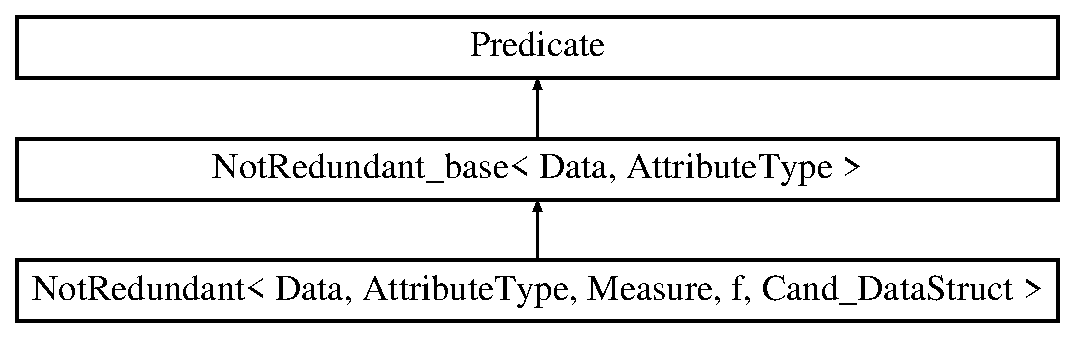
\includegraphics[height=3cm]{class_not_redundant__base}
\end{center}
\end{figure}
\subsection*{Public Member Functions}
\begin{CompactItemize}
\item 
template$<$class Input\-DBFormat$>$ {\bf Not\-Redundant\_\-base} (Data \&intable, Input\-DBFormat \&input)\label{class_not_redundant__base_4092a325b462c642b99353b33d35030b}

\begin{CompactList}\small\item\em Constructor. \item\end{CompactList}\item 
{\bf $\sim$Not\-Redundant\_\-base} ()\label{class_not_redundant__base_508fc4c9e91210a2998dfcd951c15952}

\begin{CompactList}\small\item\em Destructor. \item\end{CompactList}\item 
template$<$class Iterator, class Measure$>$ bool {\bf operator()} (Iterator itemset\-It, Measure \&mes\-Cand)
\begin{CompactList}\small\item\em Operator that test if a set of attributes is not redundant. \item\end{CompactList}\end{CompactItemize}
\subsection*{Protected Member Functions}
\begin{CompactItemize}
\item 
template$<$class Iterator$>$ void {\bf subset} (Iterator it\-Cand, int i, vector$<$ Attribute\-Type $>$ \&subset)
\begin{CompactList}\small\item\em Generate the i-th subset of size k-1 of a candidate set of size k. \item\end{CompactList}\item 
template$<$class Iterator$>$ int {\bf count\-Projection} (Iterator it\-Cand)
\begin{CompactList}\small\item\em function used to count the projection of a candidates pointed by the iterator passed in parameter. \item\end{CompactList}\end{CompactItemize}
\subsection*{Protected Attributes}
\begin{CompactItemize}
\item 
Data $\ast$ {\bf table}\label{class_not_redundant__base_332c76670be6975fddd8b7b7f52cae94}

\begin{CompactList}\small\item\em the tabular data \item\end{CompactList}\item 
{\bf Recode\-To\-Int}$<$ Attribute\-Type $>$ {\bf num\-Attrib}\label{class_not_redundant__base_9e18cbc6284d736b782c816199596f78}

\begin{CompactList}\small\item\em Used to get the numero of the attributes ( 1st, 2nd,...). \item\end{CompactList}\end{CompactItemize}
\subsection*{Classes}
\begin{CompactItemize}
\item 
class {\bf add\-Subset}
\begin{CompactList}\small\item\em Functor that adds all the elment of a container in another one, except the i th element. \item\end{CompactList}\item 
class {\bf Process\-Tuples}
\begin{CompactList}\small\item\em Functor used to projet all the tuples wrt attributes studied. \item\end{CompactList}\item 
class {\bf project}
\begin{CompactList}\small\item\em Functor used to projet a tuple wrt the set of attributes studied. \item\end{CompactList}\end{CompactItemize}


\subsection{Detailed Description}
\subsubsection*{template$<$class Data, class Attribute\-Type$>$ class Not\-Redundant\_\-base$<$ Data, Attribute\-Type $>$}

Functor representing the predicate being not redundant. 

This functor test if an itemset is not redundant. The method used to test if a canidate is not redundant is the following one: the functor process the cardinality of the projection wrt the attributes of the candidate. for each k-1 subset of the k candidates (ie with k attributes), count their projection . return false if one of the subset have the same projection cardinality that the candidate.

The template parameter Data is the type of the tablular data. The template parameter Attribute\-Type is the type of the attributes. 



\subsection{Member Function Documentation}
\index{NotRedundant_base@{Not\-Redundant\_\-base}!countProjection@{countProjection}}
\index{countProjection@{countProjection}!NotRedundant_base@{Not\-Redundant\_\-base}}
\subsubsection{\setlength{\rightskip}{0pt plus 5cm}template$<$class Data, class Attribute\-Type$>$ template$<$class Iterator$>$ int {\bf Not\-Redundant\_\-base}$<$ Data, Attribute\-Type $>$::count\-Projection (Iterator {\em it\-Cand})\hspace{0.3cm}{\tt  [protected]}}\label{class_not_redundant__base_4197a9ab9226918dba7ad6d155c9cc82}


function used to count the projection of a candidates pointed by the iterator passed in parameter. 

\begin{Desc}
\item[Parameters:]
\begin{description}
\item[{\em it\-Cand}]iterator on the candidate to test. \end{description}
\end{Desc}
\begin{Desc}
\item[Returns:]the cardinality of the projection. \end{Desc}
\index{NotRedundant_base@{Not\-Redundant\_\-base}!operator()@{operator()}}
\index{operator()@{operator()}!NotRedundant_base@{Not\-Redundant\_\-base}}
\subsubsection{\setlength{\rightskip}{0pt plus 5cm}template$<$class Data, class Attribute\-Type$>$ template$<$class Iterator, class Measure$>$ bool {\bf Not\-Redundant\_\-base}$<$ Data, Attribute\-Type $>$::operator() (Iterator {\em it\-Cand}, Measure \& {\em mes\-Cand})}\label{class_not_redundant__base_8a2f2747d1462b78140eef2a0c302d67}


Operator that test if a set of attributes is not redundant. 

\begin{Desc}
\item[Parameters:]
\begin{description}
\item[{\em it\-Cand}]iterator (or pointer) on the set of attributes to test wrt the predicate \item[{\em mes\-Cand}]cardinality of the projection on the db of the attributes \end{description}
\end{Desc}


Reimplemented from {\bf Predicate} {\rm (p.\,\pageref{class_predicate_6fb1a75dba2268f75738f335f403e46c})}.\index{NotRedundant_base@{Not\-Redundant\_\-base}!subset@{subset}}
\index{subset@{subset}!NotRedundant_base@{Not\-Redundant\_\-base}}
\subsubsection{\setlength{\rightskip}{0pt plus 5cm}template$<$class Data, class Attribute\-Type$>$ template$<$class Iterator$>$ void {\bf Not\-Redundant\_\-base}$<$ Data, Attribute\-Type $>$::subset (Iterator {\em it\-Cand}, int {\em i}, vector$<$ Attribute\-Type $>$ \& {\em subset})\hspace{0.3cm}{\tt  [protected]}}\label{class_not_redundant__base_e762398d92f03aadce4393a33dd7bc95}


Generate the i-th subset of size k-1 of a candidate set of size k. 

\begin{Desc}
\item[Parameters:]
\begin{description}
\item[{\em it\-Cand}]iterator on the candidate from wich the subset have to be generated. \item[{\em i}]number of the ignored element of the candidate to generate a k-1 subset. \item[{\em subset}]container with the subset generated. \end{description}
\end{Desc}


The documentation for this class was generated from the following file:\begin{CompactItemize}
\item 
D:/Implementations/Librairie/problems/not\-Redundant/Not\-Redundant\_\-base.hxx\end{CompactItemize}
